\chapter{Premodern Japan: Court, Samurai and Tokugawa}

\section{Early Japan}

\begin{center}
\begin{tabular}{llp{7.5cm}}
\toprule
Period & Dates & Key features \\
\midrule
Jōmon \ja{縄文} & c.\ 14\,000--300 BCE & hunter-gatherers; cord-marked pottery \\
Yayoi \ja{弥生} & c.\ 300 BCE--250 CE & wet-rice farming, bronze and iron from the continent \\
Kofun \ja{古墳} & c.\ 250--538 & giant keyhole-shaped tombs; Yamato rulers \\
Asuka \ja{飛鳥} & 538--710 & Buddhism; Prince Shōtoku; Taika reforms (645) \\
Nara \ja{奈良} & 710--794 & first permanent capital; \emph{Kojiki} (712), \emph{Nihon shoki} (720) \\
Heian \ja{平安} & 794--1185 & court aristocracy in Kyoto; Fujiwara regents; kana literature \\
Kamakura \ja{鎌倉} & 1185--1333 & first shogunate; Mongol invasions; new Buddhism \\
Muromachi \ja{室町} & 1336--1573 & Ashikaga shoguns; Zen culture; Warring States (1467--1568) \\
Azuchi--Momoyama & 1568--1600 & unifiers: Nobunaga, Hideyoshi, Ieyasu \\
Edo \ja{江戸} & 1603--1868 & Tokugawa shogunate; ``closed country''; urban culture \\
\bottomrule
\end{tabular}
\end{center}

\subsection{Selective borrowing from the continent}

The Yamato court consciously built a Chinese-style state in the 7th--8th centuries:

\begin{itemize}
  \item \textbf{Prince Shōtoku} (574--622): the Seventeen-Article Constitution (604),
        mixing Confucian and Buddhist ideals (``harmony is to be valued''); embassies to
        the Sui. A famous letter from ``the Son of Heaven where the sun rises'' to ``the Son
        of Heaven where the sun sets'' annoyed the Sui emperor, who did not accept equals.
  \item \textbf{Taika Reforms} (645 onward) and the \emph{ritsuryō} codes (701): land
        nationalized and redistributed on the Tang model, provinces, ranks, taxes.
  \item The title \emph{tennō} (\ja{天皇}, ``heavenly sovereign'') for the ruler.
\end{itemize}

\begin{important}[What Japan did \emph{not} adopt]
\begin{itemize}
  \item \textbf{Examinations}: office stayed hereditary in aristocratic clans.
  \item \textbf{The Mandate of Heaven}: the imperial line was claimed to descend unbroken
        from the sun goddess Amaterasu, so it could not lose a mandate. Instead, real
        power shifted to regents and shoguns who ruled in the emperor's name.
\end{itemize}
This is the key structural difference from China and Korea.
\end{important}

\section{Heian court culture (794--1185)}

In 894 the court stopped sending embassies to the Tang, and a period of ``national
style'' (\ja{国風文化}, kokufū bunka) followed. Politics was dominated by the
\textbf{Fujiwara} clan, who married daughters to emperors and ruled as regents for their
grandsons. Fujiwara no Michinaga (966--1028) was the peak of this power.

\subsection{Aesthetics}

\begin{itemize}
  \item \textbf{\emph{Mono no aware}} (\ja{もののあはれ}): a sensitivity to the pathos of
        things, the poignant beauty of what is transient (falling cherry blossoms).
  \item \textbf{\emph{Miyabi}} (\ja{雅}): courtly refinement; taste displayed in poetry,
        calligraphy, choice of paper and layered robe colours.
  \item Poetry (\emph{waka}, 31 syllables in 5-7-5-7-7) was the medium of courtship and
        social life. The \emph{Kokinshū} (905) was the first imperial anthology.
\end{itemize}

\subsection{Women writers}

Because men were expected to write in Chinese, the great vernacular prose of the Heian
period was written in hiragana, much of it by women of the court.

\begin{center}
\begin{tabular}{llp{6cm}}
\toprule
Work & Author & Description \\
\midrule
\emph{The Tale of Genji} \ja{源氏物語} & Murasaki Shikibu & long narrative of Prince Genji's loves; often called the first novel (c.\ 1008) \\
\emph{The Pillow Book} \ja{枕草子} & Sei Shōnagon & witty lists and observations of court life \\
\emph{Kagerō Diary} \ja{蜻蛉日記} & Mother of Michitsuna & unhappy marriage to a Fujiwara courtier \\
\bottomrule
\end{tabular}
\end{center}

\begin{aside}
Sei Shōnagon's lists (``Things that make the heart beat faster'', ``Hateful things'') read
almost like blog posts.
\end{aside}

\section{The rise of the samurai}

In the provinces, local strongmen and estate managers formed armed bands to protect
private estates (\emph{shōen}). The court used them as police and soldiers, and two great
warrior houses, the \textbf{Taira} and the \textbf{Minamoto}, became involved in court
politics. The Genpei War (1180--1185), told in the \emph{Tale of the Heike}, ended with
the Minamoto victory at Dan-no-ura.

\begin{definition}[Shogun]
\emph{Shōgun} (\ja{将軍}), short for \emph{sei-i taishōgun}, ``barbarian-subduing great
general''. Minamoto no Yoritomo received the title in 1192 and set up a military
government, the \emph{bakufu} (\ja{幕府}, ``tent government''), at Kamakura. The emperor
and court remained in Kyoto with prestige but little power.
\end{definition}

\begin{center}
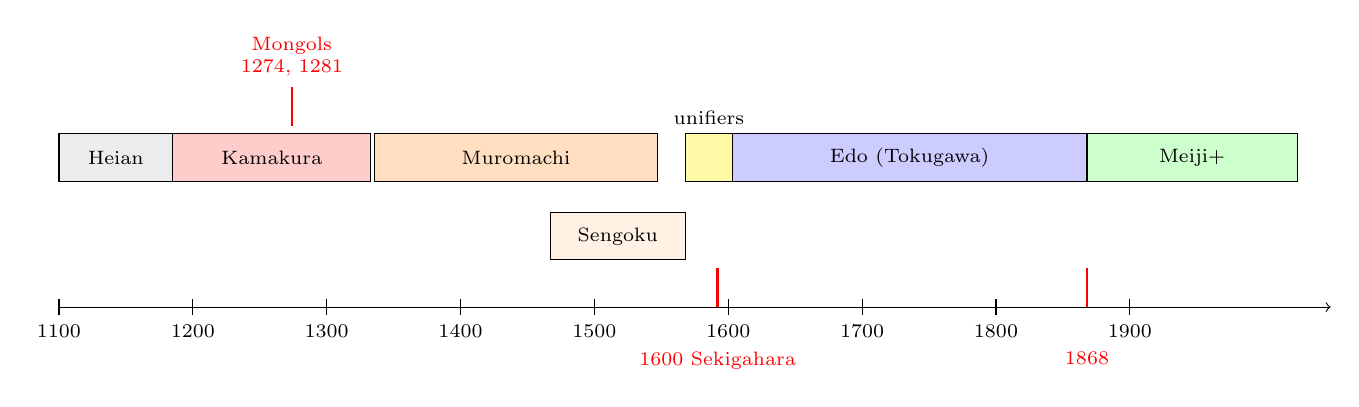
\begin{tikzpicture}[x=0.85cm, y=1cm, every node/.style={font=\scriptsize}]
  \draw[->] (0,0) -- (19,0);
  \foreach \x/\l in {0/1100, 2/1200, 4/1300, 6/1400, 8/1500, 10/1600, 12/1700, 14/1800, 16/1900} {
    \draw (\x,0.1) -- (\x,-0.1) node[below] {\l};
  }
  \draw[fill=gray!15] (0,1.6) rectangle (1.7,2.2) node[midway] {Heian};
  \draw[fill=red!20] (1.7,1.6) rectangle (4.66,2.2) node[midway] {Kamakura};
  \draw[fill=orange!25] (4.72,1.6) rectangle (8.94,2.2) node[midway] {Muromachi};
  \draw[fill=orange!10] (7.34,0.6) rectangle (9.36,1.2) node[midway] {Sengoku};
  \draw[fill=yellow!35] (9.36,1.6) rectangle (10.06,2.2);
  \draw[fill=blue!20] (10.06,1.6) rectangle (15.36,2.2) node[midway] {Edo (Tokugawa)};
  \draw[fill=green!20] (15.36,1.6) rectangle (18.5,2.2) node[midway] {Meiji+};
  \node[above] at (9.71,2.2) {unifiers};
  \draw[red, thick] (3.48,2.3) -- (3.48,2.8) node[above, align=center] {Mongols\\1274, 1281};
  \draw[red, thick] (9.84,0.5) -- (9.84,0); \node[red, below] at (9.84,-0.45) {1600 Sekigahara};
  \draw[red, thick] (15.36,0.5) -- (15.36,0); \node[red, below] at (15.36,-0.45) {1868};
\end{tikzpicture}
\end{center}

\subsection{Key episodes}

\begin{itemize}
  \item \textbf{Mongol invasions} (1274, 1281): Khubilai's fleets (with Korean ships) were
        wrecked by storms remembered as \emph{kamikaze} (\ja{神風}, ``divine winds''), a
        term revived in 1944--45.
  \item \textbf{Ashikaga shogunate} (Muromachi): Zen culture, Noh theatre, ink painting,
        the tea ceremony, rock gardens (Ryōanji), the Golden and Silver Pavilions.
  \item \textbf{Ōnin War} (1467--1477) began the \textbf{Sengoku} (``Warring States'')
        era: regional lords (\emph{daimyō}) fought constantly; ``those below overthrow those
        above'' (\ja{下克上}, gekokujō).
  \item \textbf{Europeans}: Portuguese traders reached Tanegashima in 1543 with firearms;
        Francis Xavier brought Jesuit Christianity in 1549. By 1600 there were perhaps
        300\,000 Japanese Christians.
\end{itemize}

\subsection{The three unifiers}

\begin{center}
\begin{tabular}{lp{10cm}}
\toprule
Oda Nobunaga (1534--1582) & ruthless innovator; used massed musketeers (Nagashino, 1575);
burned the Enryakuji monastery; betrayed and killed by a vassal. \\
Toyotomi Hideyoshi (1537--1598) & peasant-born; completed unification (1590); sword hunt
(1588) disarmed peasants and froze the social classes; invaded Korea (1592--98). \\
Tokugawa Ieyasu (1543--1616) & won the Battle of Sekigahara (1600); shogun 1603; his
house ruled until 1867. \\
\bottomrule
\end{tabular}
\end{center}

\begin{aside}
A famous saying contrasts them through a cuckoo that will not sing. Nobunaga: ``Kill it.''
Hideyoshi: ``Make it want to sing.'' Ieyasu: ``Wait until it sings.''
\end{aside}

\section{The Tokugawa order (1603--1868)}

\subsection{Political structure}

\begin{center}
\begin{tikzpicture}[b/.style={draw, thick, rounded corners, align=center, font=\small, minimum width=3cm}]
  \node[b, fill=yellow!20] (emp) at (-3.2,3) {Emperor (Kyoto)\\symbolic legitimacy};
  \node[b, fill=blue!20] (sh) at (2.2,3) {Shogun (Edo)\\bakufu};
  \node[b, fill=blue!10] (fu) at (-1.6,1.2) {\emph{fudai} daimyō\\(hereditary vassals)};
  \node[b, fill=red!10] (to) at (3.4,1.2) {\emph{tozama} daimyō\\(``outside'' lords)};
  \node[b, fill=gray!10] (dom) at (0.9,-0.6) {about 260 domains (\ja{藩}, han)\\each with its own samurai};
  \draw[->, thick, dashed] (emp) -- node[above, font=\scriptsize] {appoints} (sh);
  \draw[->, thick] (sh) -- (fu);
  \draw[->, thick] (sh) -- (to);
  \draw[->, thick] (fu) -- (dom);
  \draw[->, thick] (to) -- (dom);
\end{tikzpicture}
\end{center}

\begin{itemize}
  \item \textbf{Alternate attendance} (\ja{参勤交代}, sankin kōtai): daimyō spent every
        other year in Edo and left their families there as hostages. The cost kept them
        weak; the processions built roads, inns and a national culture.
  \item \textbf{Status system}: samurai, farmers, artisans, merchants (\ja{士農工商}), in
        Confucian order. In practice merchants grew rich while many samurai fell into debt.
  \item Samurai became salaried bureaucrats living in castle towns; the ideal of
        \emph{bushidō} was largely systematized in this peaceful era and romanticized
        later (Nitobe Inazō's \emph{Bushido}, 1900, written in English).
\end{itemize}

\subsection{``Closed country''}

After the Shimabara Rebellion (1637--38), a largely Christian peasant uprising, the bakufu:

\begin{itemize}
  \item banned Christianity (suspects had to trample on images, \ja{踏み絵}, fumie);
  \item forbade Japanese from travelling abroad;
  \item expelled the Portuguese, leaving only the Dutch (on the artificial island of Dejima
        in Nagasaki) and Chinese traders.
\end{itemize}

\begin{important}[\emph{Sakoku} is a misleading word]
\emph{Sakoku} (\ja{鎖国}, ``chained country'') was coined in 1801 and the policy was not
total isolation. Japan had four ``mouths'' to the outside: Nagasaki (Dutch and Chinese),
Tsushima (Korea, with Korean embassies to Edo), Satsuma (Ryukyu) and Matsumae (the Ainu).
Through ``Dutch learning'' (\ja{蘭学}, rangaku) Japanese scholars followed European
medicine and science. ``Maritime restrictions'' is a better description.
\end{important}

\subsection{Edo urban culture}

Edo (Tokyo) had over a million people by 1720, possibly the largest city in the world.
Commercial wealth produced a vibrant popular culture, the ``floating world''
(\ja{浮世}, ukiyo):

\begin{itemize}
  \item kabuki and bunraku puppet theatre (Chikamatsu Monzaemon);
  \item woodblock prints (\emph{ukiyo-e}: Hokusai's \emph{Great Wave}, Hiroshige);
  \item haiku (Matsuo Bashō, ``old pond / a frog jumps in / sound of water'');
  \item comic fiction, illustrated books, and ghost stories (see EASIA 120R).
\end{itemize}

\subsection{Intellectual currents}

\begin{itemize}
  \item \textbf{Neo-Confucianism} (Hayashi Razan) as bakufu ideology.
  \item \textbf{National Learning} (\ja{国学}, kokugaku): Motoori Norinaga (1730--1801)
        studied the \emph{Kojiki} and \emph{Genji} to recover a pure Japanese spirit before
        Chinese influence. This fed 19th-century emperor-centred nationalism.
\end{itemize}

\section*{Summary}
\begin{itemize}
  \item Japan borrowed Tang institutions selectively, rejecting exams and the Mandate of
        Heaven; the imperial line became a symbolic legitimator.
  \item Heian court culture: Fujiwara regents, kana literature by women, \emph{mono no
        aware}.
  \item Warrior rule from 1185: Kamakura, Muromachi, Sengoku, then unification by
        Nobunaga, Hideyoshi and Ieyasu.
  \item Tokugawa: alternate attendance, status system, maritime restrictions (not total
        isolation), flourishing urban culture.
\end{itemize}
